Escribe las coordenadas de los puntos indicados en el plano cartesiano de cada uno de los siguientes incisos.
	
	\begin{multicols}{2}
			\begin{parts}

				\subsubsection{Ubicación en el plano cartesiano}
				
				\part Coordenadas del punto A = \fillin[$(1,5)$][0in]
				
				\part Coordenadas del punto B = \fillin[$(-3,6)$][0in]
				
				\part Coordenadas del punto C = \fillin[$(5,-3)$][0in]
				
				\part Coordenadas del punto D = \fillin[$(-5,0$][0in]
				
				\part Coordenadas del punto E = \fillin[$(0,-7)$][0in]
				\subsubsection{Cuadrantes en el plano cartesiano}
				
				\part el punto C en el plano cartesiano: \fillin[4 cuad.][1in]
				
				\part el punto B en el plano cartesiano: \fillin[2 cuad.][1in]
				
				\part el punto A en el plano cartesiano: \fillin[1 cuad.][1in]
			\end{parts}
			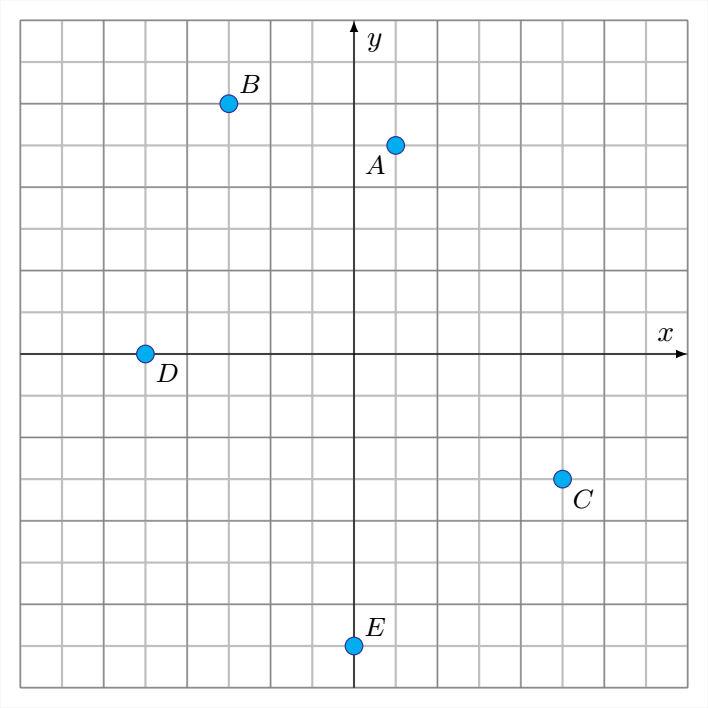
\includegraphics[width=0.8\linewidth]{../images/imagen_plano01.png}
		\end{multicols}